\documentclass[letterpaper, reqno,11pt]{article}
\usepackage[margin=1.0in]{geometry}
\usepackage{color,latexsym,amsmath,amssymb,graphicx,float,listings,tikz}
\usepackage{hyperref}

\tikzstyle{vertex}=[shape=circle, minimum size=2mm, fill, draw, inner sep=0]

\hypersetup{
colorlinks=true,
linkcolor=magenta,
filecolor=magenta,
urlcolor=cyan,
}

\graphicspath{ {images/} }

\begin{document}
\pagenumbering{arabic}
\title{Math 443 Homework 2}
\date{31/01/23}
\author{Xander Naumenko}
\maketitle

{\medskip\noindent\bf Question 1.} ($\Rightarrow$) For the forward direction, we will use proof by induction on the number of edges $n$ with the number of vertices $m$ fixed. For the base case, let $G$ be a graph with $m$ vertices and no edges. Then $\sum_{i=1}^{n}d_i=0$ which is even. For the inductive step assume that every graph with $m$ vertices and $n$ edges has an even sum of degree sequences, and let $G$ be a graph with $m$ vertices and $n+1$ edges. Let $\{x,y\}\in E(G), x,y\in V$. Then $|E(G)-\{x,y\}|=n$, so the sum of degree sequence for $G-xy$ is even. However the sum of degree sequence of $G$ is just the sum of degree sequence for $G-xy $ plus two since $\{x,y\} $ is adjacent to two vertices, so it's also even and we're done. 

($\Leftarrow$) For the backwards direction, we will construct a multigraph with the required properties. Let $d_1,\ldots,d_n$ be a sequence of nonnegative integers with $\sum_{i=1}^{n}d_i$ even. Then note that an even number of elements of $\{d_1,\ldots,d_n\}$ are even. To see why this is suppose otherwise, suppose that there were an odd number $k$ of odd elements in the sequence. Then there are $\frac{k-1}{2}$ pairs of odd numbers in the sum that add to even numbers with one left over, and since all other elements are even by assumption, the sum would be odd which is impossible. Therefore there are an even number of odd elements in the sequence. 

Since there are an even number of odd elements, consider pairing them together arbitrarily. Now consider creating a multigraph $G$. First create $n$ vertices labelled $1$ to $n$, then add an edge to between each vertex paired together with the above process. Then for each $i\in[n]$, add a number of edges of the form $\{v_i,v_i\} $ equal to either $d_i$ if $d_i$ is even, or $d_i-1$ if $d_i$ is odd. Then each vertex labeled $i$ has degree $d_i$ by construction, so $d_1,\ldots,d_n$ is a degree sequence. $\square$

{\medskip\noindent\bf Question 2.} First note that there exists at least one vertex with degree $d_1$. Since some entry in $s_1$ is negative, $\exists i\in [n]$ such that $d_i=0$. Also since only the first $d_i+1$ elements of $s_1$ are changed from $s$ it must be that $i\leq d_1+1$. Since $s$ is non-increasing this implies that $\forall j\in \{i, i+1,\ldots, n\}, d_j=0$. But then the number of non-zero entries in $s$ is smaller than $n-(n-i)=i\leq d_1+1$. This means that if $s$ were to be a degree sequence then there are strictly less than $d_1+1$ non-singleton vertices, which is clearly incompatible with there being a vertex with degree $d_1$ (since there aren't enough other non-singleton vertices to connect to). Therefore $s$ isn't graphical. $\square$

{\medskip\noindent\bf Question 3.} Suppose that the nonincreasing nonnegative integer list $s: d_1, d_2, \ldots,d_n$ is graphic, and suppose $G$ with $V(G)=\{v_1,\ldots,v_n\} $ is a graph with $s$ as it's degree sequence and with $d(v_i)=d_i$. Fix $k\in [n]$, and divide $V(G)$ into two subsets $V_1=\{v_1,\ldots,v_k\}$ and $V_2=\{v_{k+1},\ldots,v_n\}$. Also divide $E(G)$ into three subsets: $E_1=\{\{x,y\} \in E(G): x,y\in V_1\}$, $E_2=\{\{x,y\} \in E(G): x,y\in V_2\}$ and $E_3=\{\{x,y\} \in E(G): x\in V_1,y\in V_2\text{ or }x\in V_2,y\in V_1\}$. In words $E_1$ is the set of edges between the first $k$ vertices, $E_2$ is the set of edges between the remaining vertices  and $E_3$ is the set of vertices that go between the two groups. Since each element of $E_1$ adds two to the sum of degree of $V_1$, $E_2$ adds nothing and each element of $E_3$ adds one to the total degree, we have

\[
    \sum_{i=1}^{k}d_i=\sum_{v\in V_1}d(v)=2|E_1|+|E_3|
.\]
Note that a $k$-complete graph has $\frac{k(k-1)}{2}$ edges and this is the maximum number of edges that a $k$ vertex graph can have, so clearly $2|E_1|\leq k(k-1)$. Next consider $|E_3|$. This is the number of edges between $V_1$ and $V_2$, so to enumerate them we can count the number of edges each vertex of $V_2$ has to $V_1$: 
\[
    2|E_1|+|E_3|\leq k(k-1)+\sum_{i=k+1}^{n}\left| \{v\in N(v_i):v\in V_1\}  \right| 
.\]
For each $i>k$, $\left| \{v\in N(v_i):v\in V_1\}  \right|$ is clearly smaller than or equal to $d_i$ since $|N(v_i)|=d_i$, and it's also smaller than or equal to $k$ since $|V_1|=k$. Therefore $\left| \{v\in N(v_i):v\in V_1\}  \right|\leq \min(k,d_i)$. Putting this all together we get 
\[
    \sum_{i=1}^{k}d_i\leq k(k-1)+\sum_{i=k+1}^{n}\left| \{v\in N(v_i):v\in V_1\}  \right|\leq k(k-1)+\sum_{i=k+1}^{n}\min(k,d_i)
\]
as required. $\square$ 

{\medskip\noindent\bf Question 4.} Clearly adjacency matrices of undirected graphs are symmetric, since the adjacency relationship is symmetric. Thus the diagonal entries of $A^2$ are the total number of vertices adjacent to their respectively indexed vertex, which is exactly the definition of degree. So a degree sequence for $A$ is $3,3,2,2,1,1$.

{\medskip\noindent\bf Question 5.} Let $A,B,G,I$ defined as in the question. Let $V=\{v_i\in V(G): i\in I\}$. The adjacency matrix $B$ describes the same graph as $A$ except with some rows/column removed, and each row/column of index $i$ represents the vertex $v_i$. So B represents the graph $G-V$. 

{\medskip\noindent\bf Question 6.} The only possible graph is as follows:

\begin{center}
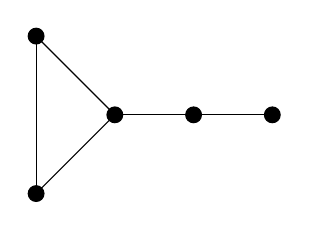
\begin{tikzpicture}
\draw (0,0)node[vertex]{};
\draw (0,2)node[vertex]{};
\draw (1,1)node[vertex]{};
\draw (2,1)node[vertex]{};
\draw (3,1)node[vertex]{};
\draw (0,0)--(0,2);
\draw (0,0)--(1,1);
\draw (0,2)--(1,1);
\draw (1,1)--(2,1);
\draw (2,1)--(3,1);
\end{tikzpicture}
\end{center}

To see why this is the only possibility, consider reconstructing the original graph. The number of nodes is $5$ and the number of edges is $\frac{1}{n-2}\sum_{i=1}^{n}| |C_i| |=\frac{15}{3}=5$ where the $C_i$ are the cards of the original graph. The first vertex-deleted subgraph tells us that the original graph must be in the form: 

\begin{center}
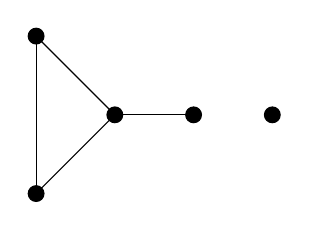
\begin{tikzpicture}
\draw (0,0)node[vertex]{};
\draw (0,2)node[vertex]{};
\draw (1,1)node[vertex]{};
\draw (2,1)node[vertex]{};
\draw (3,1)node[vertex]{};
\draw (0,0)--(0,2);
\draw (0,0)--(1,1);
\draw (0,2)--(1,1);
\draw (1,1)--(2,1);
\end{tikzpicture}
\end{center}
with one additional edge connected to the rightmost vertex. Trying all 4 possible places to put the remaining edge shows that the only one that results in two paths of length 4 is the graph shown at the beginning. 

{\medskip\noindent\bf Question 7.} The statement is true. Let $G$ be an $r$-regular graph. First note that regularity is recoverable. This follows from the fact that the degree sequence is recoverable, and a regular graph has a degree sequence of all the same numbers. Therefore the deck $D$ of $G$ implies any graph that results $D$ must be $r$-regular. 

Let $C\in D$ be an arbitrary card in the deck of $G$. Since $C$ is a vertex deleted induced subgraph, it has $|G|-1$ vertices. Also since the vertex that was deleted had degree $r$, the number of edges is $| |G| |-r$. Each of the removed edges was attached to another vertex with original degree $r$, so let $V$ be the set of vertices in $C$ with degree $r-1$. Regularity is recoverable so it must be that a reconstruction of $D$ is $r$-regular, but the only way having that be so is if each $v\in V$ is connected to the one vertex not in $V(C)$, which is exactly the graph we started with. Since this reconstruction was forced, $G$ is reconstructible (note that even though we only used a single card in the deck of $G$ to reconstruct $G$, to establish that $G$ is regular requires the entire deck). 

{\medskip\noindent\bf Question 8a.} For the first statement, recall that any subgraph of a complete graph is also complete. Thus for any choice of $3$ vertices in $V(K_{7})$, the resulting induced graph by keeping these three vertices is $K_{3}$, so $s_{k_{3}}(K_{7})\geq {7\choose 3}$. There are only ${7\choose 3}$ subgraphs of a $7$ vertex graph with $||K_{3}| |=3$ edges to begin with, so it must be that $s_{k_{3}}(K_{7})={7\choose 3}$. 

For the second statement, again consider all ${7\choose 3}$ choices of three vertices in $K_{7}$. For each of these choices we can take any two edges to connect together to form $P_{3}$ and all paths of length 2 are in this form, so we get $s_{P_{3}}(K_{7})={3\choose 2}{7\choose 3}=3{7\choose 3}$. 

{\medskip\noindent\bf Question 8b.} Let $Q$ and $G=\{v_{1}, \ldots, v_{n}\} $ be graphs with $|Q|<|G|$ and let $D=\{C_1,\ldots,C_n\} $ be the deck of $G$. Let $s^{i}_Q(G)$ be the number of subgraphs of $G$ isomorphic to $Q$ that contain $v_{i}$. Then $s_{Q}(C_i)=s_{Q}(G)-s^{i}_{Q}(G), C_i\in D$ by the definition of cards. Since each subgraph of $G$ isomorphic to $Q$ is counted $|Q|$ times over all possible $s^{i}_{Q}(G)$, $\sum_{i=1}^{n}s^{i}_{Q}(G)=|Q| s_{Q}(G)$. Summing over all $i$: 
\[
\sum_{i=1}^{n}s_{Q}(C_{i})=\sum_{i=1}^{n}(s_{Q}(G)-s^{i}_{Q}(G))=ns_{Q}(G)-|Q|s_{Q}(G)=(n-|Q|)s_{Q}(G)
.\]
Since $|Q|<|G|=n$ we can safely divide to explicitly reconstruct $s_{Q}(G)$:
\[
s_{Q}(G)=\frac{1}{n-|Q|}\sum_{i=1}^{n}s_{Q}(C_i)
.\ \square\]

{\medskip\noindent\bf Question 8c.} Suppose that $S_{Q}(G)$ is recognizable for all graphs $Q$ with $|Q|=|G|$. We will proceed by contradiction, so assume that there exist two graphs $G_1,G_2$ that both produce the same deck with $G_1,G_2$ not isomorphic. Next consider the set $S$ of all graphs with the same number of vertices and edges as $G_1,G_2$ (number of vertices and edges are recoverable so this is possible to construct just from the deck). Clearly $G_1\in S$ and $G_2\in S$, so there exists $Q\in S$ such that $s_{Q}(G_{1 /2})\neq 0$. In particular $s_{Q}(G_{1})=1$ and $s_{Q}(G_{2})=1$, since there's only one possible subgraph of a graph with the same number of vertices/edges as the original, which is the original graph. Thus $Q$ is isomorphic to both $G_1$ and $G_2$ which means they're isomorphic to one another, but this contradicts our assumption that they weren't so the reconstruction conjecture must be true. $\square$

\end{document}

